\documentclass[a4paper]{article}

\usepackage[T1]{fontenc}
\usepackage[utf8]{inputenc}
\usepackage[english]{babel}
\usepackage{csquotes}
\usepackage{listings}
\usepackage{multicol}
\lstset{language=c,frame=single,captionpos=b}
\usepackage{hyperref}
\usepackage{amsmath}
\usepackage[backend=biber, sorting=none,maxbibnames=40]{biblatex}
\renewbibmacro{in:}{}
\addbibresource{ref.bib}
\usepackage{graphicx}
\usepackage{placeins}
\usepackage[margin=2.5cm]{geometry}
\usepackage{subcaption}
\usepackage[affil-it]{authblk}
\usepackage{color}
\usepackage{amssymb,amsmath}

\begin{document}
\title{MPI Assignment: N-body Simulations}
\author{Stefano Sandonà}
\affil{Vrije Universiteit Amsterdam, Holland}
\date{}
		
\maketitle

\section{The N-body problem}
\label{sec:nbody_problem}
Given N celestial objects (bodies) with some properties (mass, initial velocity, radius, ...), the N-body problem consists on the  prediction of the individual motions of these bodies. This is done by measuring the forces that they exert on each other (Coulomb gravity,...). As a result, we obtain a simulation of the behavior of the system over time.  

\section{The sequential algorithm}
\label{sec:seq_algo}
Simplify structure:
\begin{lstlisting}
for each timestep do
	Compute forces between all bodies
	Compute new positions and velocities
\end{lstlisting}

As first thing, we have to discretize the time, so the application knows what to do at certain timestamps. Than for each step, the algorithm computes all the forces between all the bodies. With the resulting forces, the new velocity and positions of all the bodies are updated.

\subsection{Force computation}
\label{sec:force_comp_seq}
This step of the algorithm is the most expensive and determine its complexity.
The forces that bodies exert on each other has to be calculated once per pair of bodies.
\begin{lstlisting}
for (b=0; b<bodyCt; ++b) {
		for (c=b+1; c<bodyCt; ++c) {
			...
\end{lstlisting}
That means with N bodies, we have (N-1)+(N-2)+(N-3)+...+1 pairs, so O(N\textsuperscript{2}) force computations for every timestamp.

\section{Parallel N-body algorithm}
\label{sec:par}
An efficient parallelization of this algorithm is not trivial because for every step we need updated informations from all bodies that are part of our system to calculate the new values. 

\subsection{Bodies distribution}
\label{sec:bodies_distr}
One of the major problems of the parallel algorithms is the load imbalance. If we don't distribute the work fairly between the machines involved in the computation, we'll have some machines idle while others will still work. This problem affects a lot the performance of the application because the overall execution time depends on the last machine that terminate the computation. As each body has to interact with all the others, we have the same amount of work per body, so we just have to find a way to distribute equally the N bodies among all machines. Using a simple \textit{for} construct we can calculate the chunks of bodies to assign to each computational node (number of bodies per node and the boundaries of the chunks).

\begin{lstlisting}
int sum = 0;
for (i = 0; i < numprocs; i++) {
    bodies_per_proc[i] = bodyCt / numprocs;
    if (rem > 0) {
        bodies_per_proc[i]++;
        rem--;
    }
    displs[i] = sum;
    sum += bodies_per_proc[i];
}
\end{lstlisting}

\begin{figure}[ht]
  \centering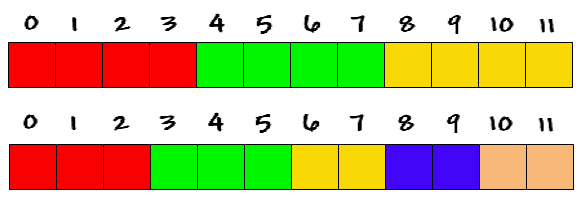
\includegraphics[width=0.6\linewidth]{array_procs_both}
  \caption{12 bodies and 3 computational nodes, 12 bodies and 5 computational nodes}
  \label{fig:3nodes}
\end{figure}
\FloatBarrier

\subsection{The Work repartition}
\label{sec:work_rep}

\subsubsection{Naive repartition}
\label{sec:naive_rep}

This is the most critical part of the implementation, from this depends the efficiency of the whole algorithm. 
Using a naive approach for every step we could simply use the MPI\_Allgatherv operation, to send to all other nodes our updated chunk of bodies and receive all the other chunks from other nodes. Than compute the forces that all other bodies exert on the actual chunk and update the actual chunk bodies positions and speeds. 

A problem of this approach is the big amount of data transferred in each iteration (N bodiesType structures) and the fact that we are computing the same forces between some pairs of bodies in more than one machine. In fact, computing the force that the body A exert on the body B, implicitly we are computing also the force that the body B exert on the body A (force of B on A is negative of A on B). Given a situation like the one described on Figure \ref{fig:nodes}, we can see on Tables \ref{table:t1} and \ref{table:t2} the forces computed by the first two nodes.

\begin{figure}[ht]
  \centering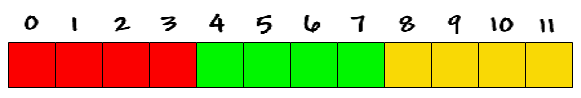
\includegraphics[width=0.6\linewidth]{array_procs_3}
  \caption{12 bodies and 3 computational nodes}
  \label{fig:nodes}
\end{figure}
\FloatBarrier

\begin{table}[]
\centering
\caption{Node 0 - Calculated forces}
\label{table:t1}
\begin{tabular}{l|lllllllllll}
bodies{[}0{]} & 0-1 & 0-2 & 0-3 & \textcolor{red}{0-4} & \textcolor{red}{0-5} & \textcolor{red}{0-6} & \textcolor{red}{0-7}  & 0-8  & 0-9  & 0-10 & 0-11 \\ \hline
bodies{[}1{]} & 1-2 & 1-3 & \textcolor{red}{1-4} & \textcolor{red}{1-5} & \textcolor{red}{1-6} & \textcolor{red}{1-7} & 1-8  & 1-9  & 1-10 & 1-11 &      \\ \hline
bodies{[}2{]} & 2-3 & \textcolor{red}{2-4} & \textcolor{red}{2-5} & \textcolor{red}{2-6} & \textcolor{red}{2-7} & 2-8 & 2-9  & 2-10 & 2-11 &      &      \\ \hline
bodies{[}3{]} & \textcolor{red}{3-4} & \textcolor{red}{3-5} & \textcolor{red}{3-6} & \textcolor{red}{3-7} & 3-8 & 3-9 & 3-10 & 3-11 &      &      &   
\end{tabular}
\end{table}

\begin{table}[]
\centering
\caption{Node 1 - Calculated forces}
\label{table:t2}
\begin{tabular}{l|lllllllllll}
bodies{[}4{]} & \textcolor{red}{4-0} & \textcolor{red}{4-1} & \textcolor{red}{4-2} & \textcolor{red}{4-3} & 4-5 & 4-6 & 4-7  & 4-8  & 4-9  & 4-10 & 4-11 \\ \hline
bodies{[}5{]} & \textcolor{red}{5-0} & \textcolor{red}{5-1} & \textcolor{red}{5-2} & \textcolor{red}{5-3} & 5-6 & 5-7 & 5-8  & 5-9  & 5-10 & 5-11 &      \\ \hline
bodies{[}6{]} & \textcolor{red}{6-0} & \textcolor{red}{6-1} & \textcolor{red}{6-2} & \textcolor{red}{6-3} & 6-7 & 6-8 & 6-9  & 6-10 & 6-11 &      &      \\ \hline
bodies{[}7{]} & \textcolor{red}{7-0} & \textcolor{red}{7-1} & \textcolor{red}{7-2} & \textcolor{red}{7-3} & 7-8 & 7-9 & 7-10 & 7-11 &      &      &     
\end{tabular}
\end{table}

As we can notice from Tables \ref{table:t1} and \ref{table:t2}, forces between the pairs highlighted in red are calculated by both Node 0 and Node 1. For each node we calculate the forces for 38 pairs, that means 114 pairs (38 x 3) in total. The number of possible pairs is 66, so we are doing about 1.7 times the needed work. 
The detailed computation is explained on the Equation \ref{eq:eq1}). 

\begin{equation} 
\label{eq:eq1}
\begin{split}
Computation & = O(\lceil\frac{N}{P}\rceil * \lceil\frac{N}{P}\rceil * (P-1)) + O((\lceil\frac{N}{P}\rceil-1)!)\\
 & = O(\frac{N^2}{P})
\end{split}
\end{equation}

With this approach for each iteration we send O(N/P) bodies and we receive O(N-N/P) bodies, that means an O(N) communication. For the computation we have the O(N\textsuperscript{2}/2P) for the force computation, and an O(N-N/P)for each the velocities and the positions computation.

\subsubsection{Optimized repartition}
\label{sec:opt_rep}
The aim of a good repartition is to not repeat the same work on different nodes. Following this objective the idea is, given a pair of chuncks, half of the forces that two bodies from different chunks exert on each other are calculated by one node, and half by the other. The ripartition is clarify on the Figures \ref{fig:pr1}, \ref{fig:pr2} and \ref{fig:pr3}.


\begin{figure}[ht]
\centering
\begin{subfigure}{.45\textwidth}
  \centering
  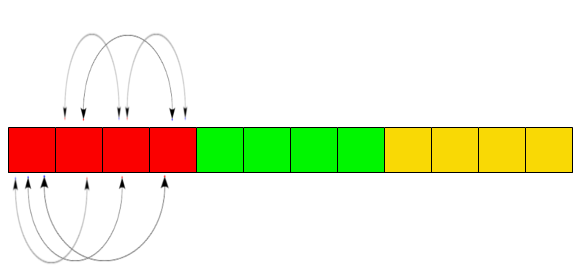
\includegraphics[width=1\linewidth]{array_proc_0_b_0}
\end{subfigure}%
\begin{subfigure}{.45\textwidth}
  \centering
  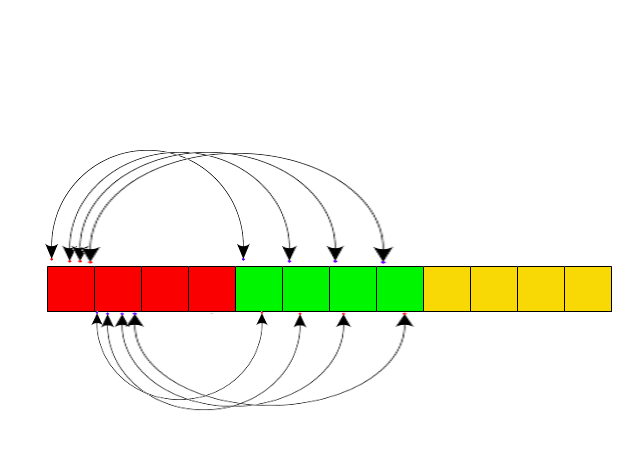
\includegraphics[width=1\linewidth]{array_proc_0_b_1}
\end{subfigure}\\ %
\begin{subfigure}{.45\textwidth}
  \centering
  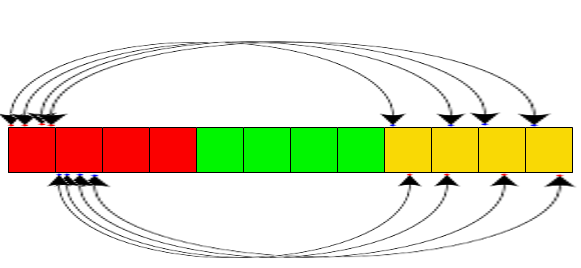
\includegraphics[width=1\linewidth]{array_proc_0_b_2}
\end{subfigure}
  \caption{Forces computed by Node 0 (6+8+8=22)}
  \label{fig:pr1}
\end{figure}
\FloatBarrier


\begin{figure}[ht]
\centering
\begin{subfigure}{.45\textwidth}
  \centering
  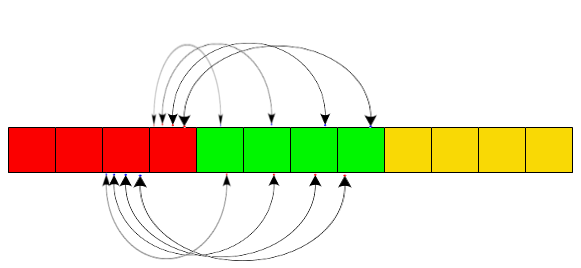
\includegraphics[width=1\linewidth]{array_proc_1_b_0}
\end{subfigure}%
\begin{subfigure}{.45\textwidth}
  \centering
  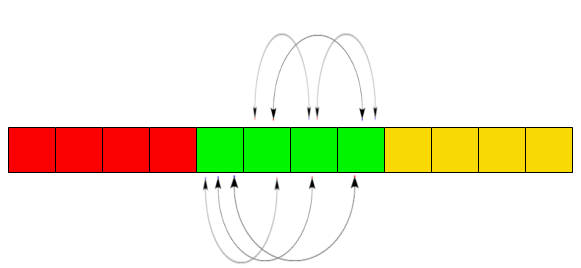
\includegraphics[width=1\linewidth]{array_proc_1_b_1}
\end{subfigure}\\ %
\begin{subfigure}{.45\textwidth}
  \centering
  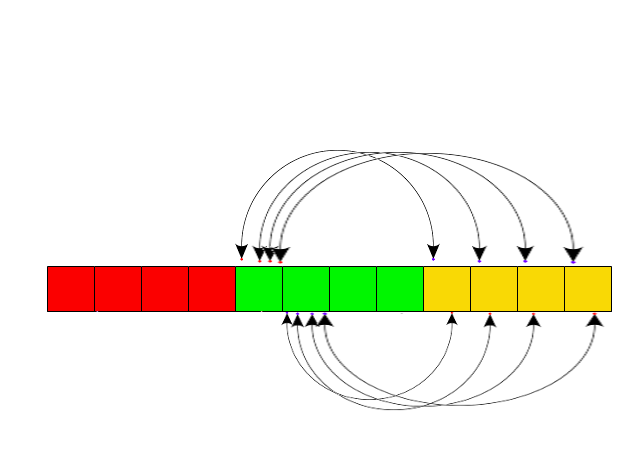
\includegraphics[width=1\linewidth]{array_proc_1_b_2}
\end{subfigure}
  \caption{Forces computed by Node 1 (8+6+8=22)}
  \label{fig:pr2}
\end{figure}
\FloatBarrier


\begin{figure}[ht]
\centering
\begin{subfigure}{.45\textwidth}
  \centering
  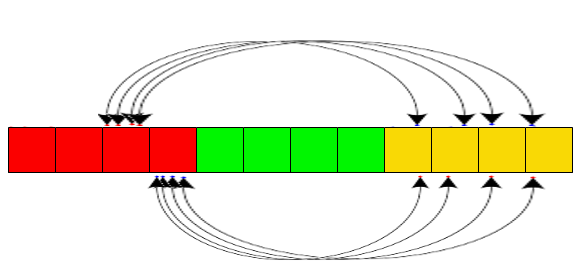
\includegraphics[width=1\linewidth]{array_proc_2_b_0}
\end{subfigure}%
\begin{subfigure}{.45\textwidth}
  \centering
  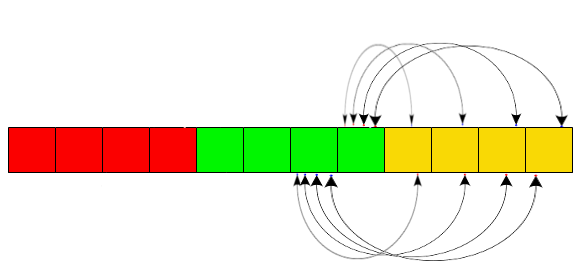
\includegraphics[width=1\linewidth]{array_proc_2_b_1}
\end{subfigure}\\ %
\begin{subfigure}{.45\textwidth}
  \centering
  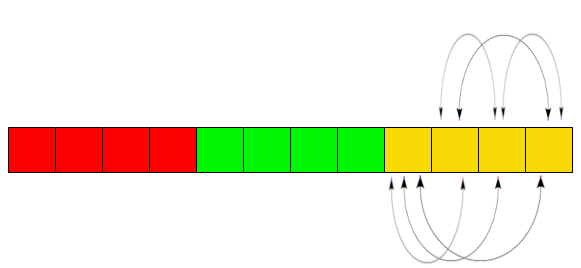
\includegraphics[width=1\linewidth]{array_proc_2_b_2}
\end{subfigure}
  \caption{Forces computed by Node 2 (8+8+6=22)}
  \label{fig:pr3}
\end{figure}
\FloatBarrier

Proceeding in this way, the forces between pairs of bodies are calculated only one time per step. Each node computes the forces of 22 pairs. We have 3 nodes, so 3 times 22 is 66 that correspond to the number of possible pairs. No useful work is done. The computational time is explained in the Equation \ref{eq:eq2}.

\begin{equation} \label{eq:eq2}
\begin{split}
Complexity & = O(\lceil\frac{N}{P}\rceil * (\lceil\frac{N}{P}\rceil * \frac{1}{2}) * (P-1)) + O((\lceil\frac{N}{P}\rceil-1)!)\\
 & = O(\frac{N^2}{2P})
\end{split}
\end{equation}

\subsection{The final solution}
\label{sec:comm_comp}

\subsubsection{Communication VS Computation}
\label{sec:comm_comp}
The communication is a common bottleneck on lots of parallel implementations. The data exchange between nodes should be reduced at the minimum in order to obtain good performances. The problem with the N body algorithm is that at every step we need the updated information (positions, velocities) of all other bodies of the system in order to correctly compute the forces of the assigned chunk. That means an exchange of data for every step. To gain performances we have to find a good compromise between the data exchange and the work to do on each node. In particular, we have to maximize the ratio \textit{computation/communication}. Due to the fact that the force computation is the most expensive part of the algorithm and that we want to exhange as less data as possible, a good compromise is the following. At the begin, we broadcast to all the nodes the bodies (MPI_Bcast). Than for each step, each node calculates the forces for the assigned pairs (the one described on Section \ref{sec:opt_rep}), after that uses an MPI_Allreduce operation to sum all the calculated forces by all the nodes and as last thing it computes the velocities and positions for all the bodies. The major problem of this approach, is that we calculate the positions and velocities of bodies in every node, that represent a duplication of work. An alternative could be to calculate in each node only the velocities and the positions of the bodies of the assigned chunk, but doing this we have to share with the other nodes also this information. The decision so, is between computing the N velocities and positions in all the nodes or exchange more data with the other nodes. 

\subsubsection{2 solutions comparison}
\label{sec:sol_comp}
After a comparison of the two solutions for different size of inputs (steps and number of bodies), it's clear that the amount of data exhanged is the key point. The Figure \ref{} shows just one example in which we can see how the execution time of the first approach is lower than the execution time on the other.




\begin{figure}[ht]
  \centering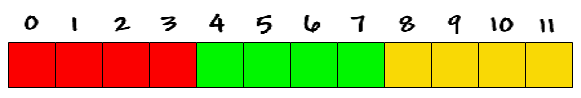
\includegraphics[width=0.6\linewidth]{array_procs_3}
  \caption{12 bodies and 3 computational nodes}
  \label{fig:3nodes}
\end{figure}
\FloatBarrier

\begin{table}[]
\centering
\caption{Node 0}
\label{my-label}
\begin{tabular}{l|llllllll}
block0 & 0-1 & 0-2 & 0-3  & 1-2  & 1-3 & 2-3 &      &      \\ \hline
block1 & 0-4 & 0-5 & 0-6  & 0-7  & 1-4 & 1-5 & 1-6  & 1-7  \\ \hline
block2 & 0-8 & 0-9 & 0-10 & 0-11 & 1-8 & 1-9 & 1-10 & 1-11
\end{tabular}
\end{table}

\begin{table}[]
\centering
\caption{Node 1}
\label{my-label}
\begin{tabular}{l|llllllll}
block0 & 2-4 & 2-5 & 2-6  & 2-7  & 3-4 & 3-5 & 3-6  & 3-7  \\ \hline
block1 & 4-5 & 4-6 & 4-7  & 5-6  & 5-7 & 6-7 &      &      \\ \hline
block2 & 4-8 & 4-9 & 4-10 & 4-11 & 5-8 & 5-9 & 5-10 & 5-11
\end{tabular}
\end{table}

\begin{table}[]
\centering
\caption{Node 2}
\label{my-label}
\begin{tabular}{l|llllllll}
block0 & 2-8 & 2-9  & 2-10 & 2-11 & 3-8  & 3-9   & 3-10 & 3-11 \\ \hline
block1 & 6-8 & 6-9  & 6-10 & 6-11 & 7-8  & 7-9   & 7-10 & 7-11 \\ \hline
block2 & 8-9 & 8-10 & 8-11 & 9-10 & 9-11 & 10-11 &      &     
\end{tabular}
\end{table}

\begin{figure}[ht]
  \centering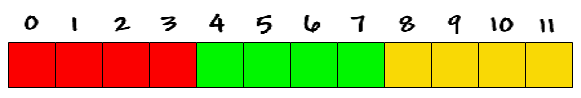
\includegraphics[width=0.6\linewidth]{array_procs_3}
  \caption{12 bodies and 5 computational nodes}
  \label{fig:5nodes}
\end{figure}

\begin{table}[]
\centering
\caption{Node 0}
\label{my-label}
\begin{tabular}{l|llllll}
block0 & 0-1  & 0-2  & 1-2 &  &  &  \\ \hline
block1 & 0-3  & 0-4  & 0-5 &  &  &  \\ \hline
block2 & 0-6  & 0-7  &     &  &  &  \\ \hline
block3 & 0-8  & 0-9  &     &  &  &  \\ \hline
block4 & 0-10 & 0-11 &     &  &  &  
\end{tabular}
\end{table}

\begin{table}[]
\centering
\caption{Node 1}
\label{my-label}
\begin{tabular}{l|llllll}
block0 & 1-3  & 1-4  & 1-5 & 2-3 & 2-4 & 2-5  \\ \hline
block1 & 3-4  & 3-5  & 4-5 &     &     &      \\ \hline
block2 & 3-6  & 3-7  &     &     &     &      \\ \hline
block3 & 3-8  & 3-9  &     &     &     &      \\ \hline
block4 & 3-10 & 3-11 &     &     &     &      
\end{tabular}
\end{table}

\begin{table}[]
\centering
\caption{Node 2}
\label{my-label}
\begin{tabular}{l|llllll}
block0 & 1-6  & 1-7  & 2-6 & 2-7 &  &  \\ \hline
block1 & 4-6  & 4-7  & 5-6 & 5-7 &  &  \\ \hline
block2 & 6-7  &      &     &     &  &  \\ \hline
block3 & 6-8  & 6-9  &     &     &  &  \\ \hline
block4 & 6-10 & 6-11 &     &     &  & 
\end{tabular}
\end{table}

\begin{table}[]
\centering
\caption{My caption}
\label{my-label}
\begin{tabular}{l|llllll}
block0 & 1-8  & 1-9  & 2-8 & 2-9 &  &  \\ \hline
block1 & 4-8  & 4-9  & 5-8 & 5-9 &  &  \\ \hline
block2 & 7-8  & 7-9  &     &     &  &  \\ \hline
block3 & 8-9  &      &     &     &  &  \\ \hline
block4 & 8-10 & 8-11 &     &     &  & 
\end{tabular}
\end{table}

\begin{table}[]
\centering
\caption{Node 3}
\label{my-label}
\begin{tabular}{l|llllll}
block0 & 1-10  & 1-11 & 2-10 & 2-11 &  &  \\ \hline
block1 & 4-10  & 4-11 & 5-10 & 5-11 &  &  \\ \hline
block2 & 7-10  & 7-11 &      &      &  &  \\ \hline
block3 & 9-10  & 9-11 &      &      &  &  \\ \hline
block4 & 10-11 &      &      &      &  & 
\end{tabular}
\end{table}

\printbibliography 

\end{document}